\documentclass[final]{beamer}

\usepackage[orientation=portrait, size=a0, scale=1.4, debug]{beamerposter}
\usepackage{booktabs}
\usepackage{dcolumn}
\usepackage{colortbl}
\usepackage{xcolor}
\usepackage{hyperref}
\usepackage{amsmath}
\usepackage[absolute, showboxes, overlay]{textpos}
%\usepackage[absolute, overlay]{textpos}
\usepackage{calc}
%\usepackage[colorgrid,texcoord]{eso-pic}
\usepackage[bibstyle=numeric]{biblatex}
% \usepackage{enumitem}
% \defaultfontfeatures{Mapping=tex-text}
\usepackage{algorithm}
\usepackage[noend]{algpseudocode} 

\usetheme{enziteto}

\addbibresource{../referomnia/referomnia.bib}

\usepackage{blindtext}

\newcommand*\mccol[2]{\multicolumn{#1}{c}{#2}}
\newcommand*\tmccol[2]{\mccol{#1}{\tiny\textsf{#2}}}
\newcommand*\bmccol[2]{\mccol{#1}{\textbf{#2}}}


% 
% custom colors
\definecolor{untractable_red}{RGB}{209, 25, 25}
\definecolor{tractable_green}{RGB}{0, 153, 51}


\setbeamertemplate{itemize item}{\raisebox{.21ex}{\hbox{\tiny\textcolor{lacamlilac}{$\boldsymbol{\oplus}$}}\hspace{0pt}}}
\setbeamertemplate{itemize subitem}{\raise .2ex\hbox{\tiny\textcolor{lacamlilac}{$\boldsymbol{\otimes}$}}\hspace{0pt}}
\setbeamertemplate{itemize subsubitem}{\textcolor{lacamlilac}{$\oplus$}}
% \setbeamertemplate{bibliography item}{\hspace{10pt}\raise
%   .2ex\hbox{\tiny\textcolor{lacamlilac}{$\boldsymbol{\oplus}$}}\insertbiblabel}
\setbeamertemplate{bibliography item}{\insertbiblabel}


\setbeamertemplate{headline}{}

% \addbibresource{../referomnia/referomnia.bib}

\title{Towards Representation Learning with Tractable Probabilistic Models}
\author{Antonio  Vergari, Nicola  {Di Mauro} and Floriana Esposito}
\date{}


\begin{document}

\institute{Università degli Studi di Bari}
\department{Dipartimento di Informatica}
\laboratory{LACAM}
\group{Machine Learning}
\institutelogo{
\includegraphics[width=25pt]{figures/unibaba}}
\lablogo{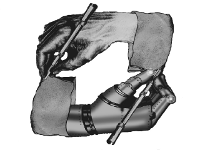
\includegraphics[width=35pt]{figures/lacam}}


% {
%   \setbeamertemplate{headline}{}
%   \setbeamertemplate{footline}{}
%   \begin{textblock}
%     \titlepage
%   \end{textblock}
% }

\newcommand{\hmargin}{20mm}
\newcommand{\vmargin}{20mm}
\textblockorigin{\hmargin}{\vmargin}

\setlength{\TPHorizModule}{1cm}
\setlength{\TPVertModule}{1cm}

%
% TODO: generalize this
\newlength{\posterwidth}
\setlength{\posterwidth}{841mm - 2\hmargin}
\newlength{\posterheight}
\setlength{\posterheight}{1189mm}

\newcommand{\ncols}{3}
\newlength{\colwidth}
\setlength{\colwidth}{\posterwidth/\ncols}


\newlength{\colhpoint}


\begin{frame}{}
  %
  % title
  % \textblockcolour{header}
  \begin{textblock}{58}(0, 0)
    \usebeamerfont{section name}
    \huge
    Towards Representation Learning\\
    with Tractable Probabilistic Models
  \end{textblock}
  %
  % authors
  \begin{textblock}{30}(0, 6.5)
    \usebeamerfont{author}
    \small
    Antonio  Vergari, Nicola  {Di Mauro} and Floriana Esposito
  \end{textblock}
  % 
  % email
  \begin{textblock}{15}(30, 6.5)
    \usebeamerfont{author}
    \small
    \emph{\{firstname.lastname@uniba.it\}}
  \end{textblock}
  %
  % affiliations
  \begin{textblock}{30}(60, 0)
    \usebeamerfont{author}
    \footnotesize
    \begin{minipage}[t]{5cm}
      \vspace{0pt}\hspace{5pt}
      
\includegraphics[width=97pt]{figures/unibaba}
    \end{minipage}\hspace{-15pt}
    \begin{minipage}[t]{15cm}
    \vspace{20pt}
      \flushleft
      University of Bari "Aldo Moro", Italy\\
    \vspace{2pt}
      Department of Computer Science
    \end{minipage}\\[0.75cm]
    \usebeamerfont{author}
    \footnotesize
    \begin{minipage}[t]{5cm}
      \vspace{0pt}
      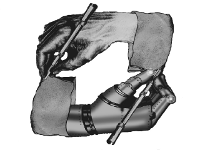
\includegraphics[width=117pt]{figures/lacam}
    \end{minipage}\hspace{-15pt}
    \begin{minipage}[t]{15cm}
      \vspace{23pt}
      \flushleft
      LACAM Laboratory\\
      \vspace{2pt}
      Machine Learning
    \end{minipage}
  \end{textblock}
  
  
  %
  % section 1
  \begin{textblock}{80}(0, 10.5)
    \usebeamerfont{section name}
    Tractable Probabilistic Models
  \end{textblock}
  
  
  \begin{textblock}{25.2}(0, 13)
    \small
    \emph{\textbf{Density estimation}} is the unsupervised task of
    learning an estimator for the joint probability distribution
    $p(\mathbf{X})$ from a set of i.i.d. samples $\{\mathbf
    x_i\}_{i=1}^m$ over RVs $\mathbf{X}$\\[20pt]
    
    Once such a density estimator is learned, one uses it to answers
    probabilistic queries about configurations on $p(\mathbf{X})$,
    that is to do\emph{\textbf{inference}}\\[20pt]
    
    Operations that may be required to be efficient are
    \begin{itemize}
    \item $p(\mathbf{X} = \mathbf{x})$ (evidence) 
    \item $p(\mathbf{E}), \mathbf{E}\subset\mathbf{X}$ (marginals)
    \item $p(\mathbf{Q}|\mathbf{E}), \mathbf{Q},
      \mathbf{E}\subset\mathbf{X}, \mathbf{Q}\cap \mathbf{E}=\emptyset$
      (conditionals)
    \item $\arg\max_{\mathbf{q}\sim\mathbf{Q}}p(\mathbf{q}|\mathbf{E})$
      (MPE assignment)
    \item $Z =\sum_{\mathbf{x}\sim \mathbf{X}}\phi(\mathbf{x})$
      (partition function)
      % \item sampling: generate independent samples from the posterior distribution
    \end{itemize}
    
  \end{textblock}
  
  \begin{textblock}{25.2}(27.4, 13)
    \small
    \emph{\textbf{Tractable Probabilistic Models}}  (\textbf{TPMs})
    are density estimators for which some kind of inference is
    \emph{tractable}, i.e. polynomial in the number of r.v.s or their domains.
  \end{textblock}

  % \begin{textblock}{25}(34.1, 15.3)
  %   \small
  %     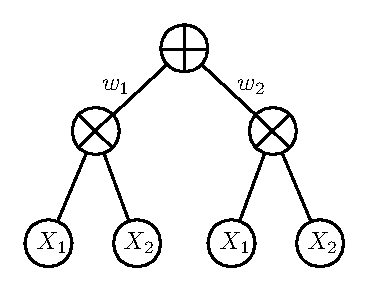
\includegraphics[width=0.7\linewidth]{figures/spn-sum}
  % \end{textblock}
  
  \begin{textblock}{25.2}(54.8, 13)
    \footnotesize
    \begin{minipage}{0.7\linewidth}
      
    Bottom-up evaluation of the network:
    $$S_{X_i}(x_j)=P(X_i=x_j)$$    
    $$S_{+}(\mathbf{x})=\sum\limits_{i\in
      ch(+)}w_{i}S_{i}(\mathbf{x})\quad S_{\times}(\mathbf{x})=\prod\limits_{i\in
      ch(\times)}S_{i}(\mathbf{x})$$\\[10pt]
    \setlength{\leftmargini}{30pt}
    Inferences linear in the \emph{\textbf{size of the network}} (\emph{\# edges}):
    \begin{itemize}
    \item $Z = S(*)$ (all leaves output 1)
    \item $P(\mathbf{e}) = S(\mathbf{e})/S(*)$
    \item $P(\mathbf{q}| \mathbf{e}) = \frac{P(\mathbf{q},
        \mathbf{e})}{P(\mathbf{e})} = \frac{S(\mathbf{q},
        \mathbf{e})}{S(\mathbf{e})}$
    \item $MPE(\mathbf{q},\mathbf{e}) = \max_{\mathbf{q}}P(\mathbf{q},
      \mathbf{e}) = S^{max}(\mathbf{e})$, turning sum nodes into max nodes
    \end{itemize}
  \end{minipage}\begin{minipage}{0.28\linewidth}
    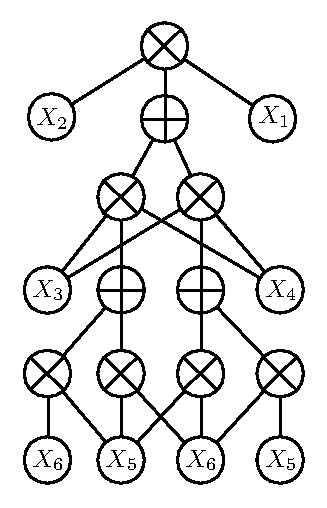
\includegraphics[width=0.8\linewidth]{figures/spn-long}
  \end{minipage}\\[20pt]

  The \emph{\textbf{depth of the network}} (\emph{\# layers})
  determines expressive efficiency~\parencite{Martens2014}.
  
  \end{textblock}
  
  %mixture
  % section 2
  \begin{textblock}{80}(0, 33.8)
    \usebeamerfont{section name}
    Representation Learning with TPMs
  \end{textblock}
  
  \begin{textblock}{25.2}(0, 36.3)
    \footnotesize
     
    SPN structure learning is a constraint-based
    search. Main ideas: to discover hidden variables for sum nodes and independences
    for product nodes by applying some form of clustering
    along matrix axis. Different variations:
    using K-Means on
    features~\emph{\parencite{Dennis2012}}; merging features bottom-up
    with IB heuristics\emph{~\parencite{Peharz2013}};
    \emph{\textbf{LearnSPN}}~\emph{\parencite{Gens2013}} is the first principled top-down greedy
    algorithm. 
    

    % \begin{itemize}
    %   \itemsep 6pt
    % \item greedy top-down: KMeans on features~\emph{\parencite{Dennis2012}};
      
    % \item greedy bottom up: merging feature regions by a \emph{Bayesian-Dirichlet independence test},  and reducing edges by maximizing MI\emph{~\parencite{Peharz2013}}

    % \item \textbf{ID-SPN}: turning LearnSPN in log-likelihood guided expansion of sub-networks
    %   approximated by Arithmetic Circuits~\emph{\parencite{Rooshenas2014}}
      
    % \end{itemize}
  \end{textblock}
  
  \begin{textblock}{25.2}(27.4, 36.3)
    \footnotesize
    LearnSPN builds a tree-like SPN by recursively splitting the data
    matrix: columns in pairs by a greedy \textbf{\emph{G Test}} based
    procedure with threshold $\rho$: $G(X_i, X_j) =  2\sum_{x_i \sim
      X_i}\sum_{x_j \sim X_j}c(x_i, x_j)\cdot \log\frac{c(x_i,
      x_j)\cdot |T|}{c(x_i)c(x_j)}$ (Figure 1.c); instances in
    $|C|$ clusters with \textbf{\emph{online Hard-EM}} (Figure 1.b) with cluster number penalty
    $\lambda$: $Pr(\mathbf{X})= \sum_{C_i \in \mathbf{C}}\prod_{X_j
      \in \mathbf{X}}Pr(X_j,C_i)$. Weights are the cluster proportions.
    
    % \begin{itemize}
    % \item splitting columns in pairs by a greedy \textbf{\emph{G Test}} based
    %   procedure with threshold $\rho$:
    %   \[
    %   G(X_i, X_j) =  2\sum_{x_i \sim X_i}\sum_{x_j \sim X_j}c(x_i, x_j)\cdot \log\frac{c(x_i, x_j)\cdot |T|}{c(x_i)c(x_j)}
    %   \]
 
    %   \end{itemize}
  \end{textblock}
  
  
  % \begin{textblock}{60}(0, 36.3)
  %   \small
  %   \begin{minipage}[t][][t]{5.103cm}
  %     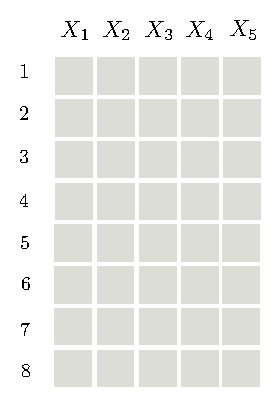
\includegraphics[width=\linewidth]{figures/grid-0}
  %   \end{minipage}\hspace{30pt}\begin{minipage}[t]{4.4874cm}
  %     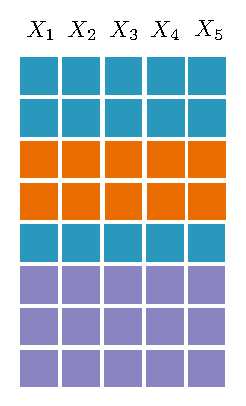
\includegraphics[width=\linewidth]{figures/grid-1}
  %   \end{minipage}\hspace{30pt}\raisebox{82pt}{\begin{minipage}[t]{5.67cm}\vspace{-120pt}
  %     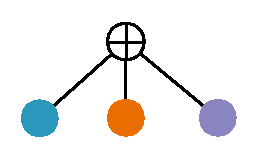
\includegraphics[width=\linewidth]{figures/learnspn-1}
  %   \end{minipage}}\hspace{30pt}\begin{minipage}[t]{4.4874cm}
  %     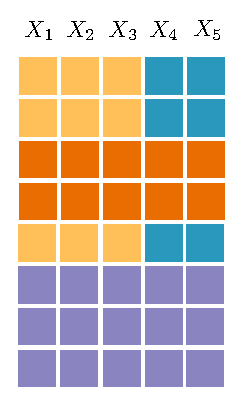
\includegraphics[width=\linewidth]{figures/grid-2}
  %   \end{minipage}\hspace{30pt}\raisebox{42pt}{\begin{minipage}[t]{6.48cm}
  %     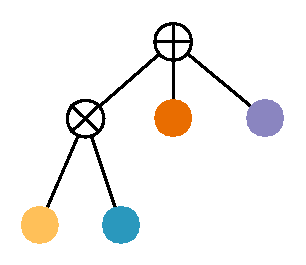
\includegraphics[width=\linewidth]{figures/learnspn-2}
  %   \end{minipage}}\hspace{30pt}\begin{minipage}[t]{4.6364cm}
  %   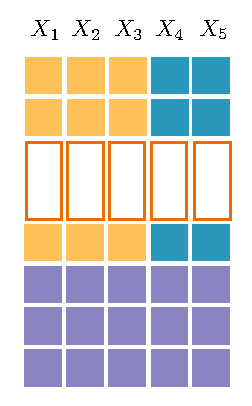
\includegraphics[width=\linewidth]{figures/grid-3}                                                               \end{minipage}\hspace{30pt}\raisebox{42pt}{\begin{minipage}[t]{8.1cm}
  %     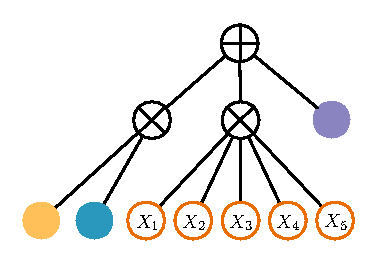
\includegraphics[width=\linewidth]{figures/learnspn-3}                                             
  %   \end{minipage}}\hspace{50pt}\raisebox{180pt}{\begin{minipage}[t]{4cm}
  %     \tiny\flushleft
  %     Figure 1.\\
  %     LearnSPN steps depiction: starting from a full data matrix \emph{(a)},
  %     clustering on rows \emph{(b)}, then on columns \emph{(c)}, and putting a naive
  %     factorization on leaves \emph{(d)}.
  %   \end{minipage}}\\
  % \vspace{-20pt}\hspace{80pt}\begin{minipage}[t]{7cm}
  %   \scriptsize\emph{(a)}
  % \end{minipage}\hspace{80pt}\begin{minipage}[t]{7cm}
  %   \scriptsize\emph{(b)}
  % \end{minipage}\hspace{175pt}\begin{minipage}[t]{7cm}
  %   \scriptsize\emph{(c)}
  % \end{minipage}\hspace{175pt}\begin{minipage}[t]{7cm}
  %   \scriptsize\emph{(d)}
  % \end{minipage}
    
  %   % \begin{table}[ht]
  %   %   \centering
  %   %   \begin{tabular}{l l l l l l l}
  %   %     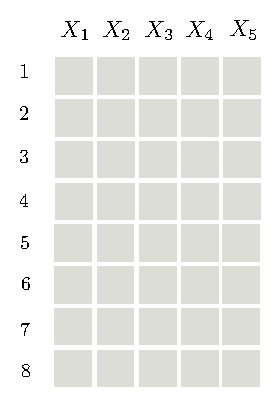
\includegraphics[width=0.228\linewidth]{figures/grid-0}&
  %   %     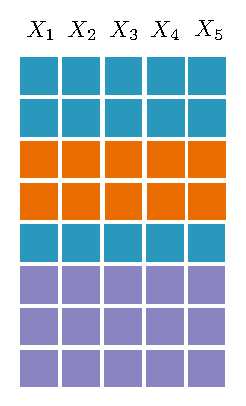
\includegraphics[width=0.2\linewidth]{figures/grid-1}&
  %   %     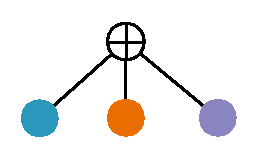
\includegraphics[width=0.2\linewidth]{figures/learnspn-1}&                                                       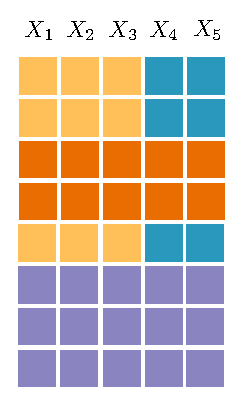
\includegraphics[width=0.2\linewidth]{figures/grid-2}&
  %   %     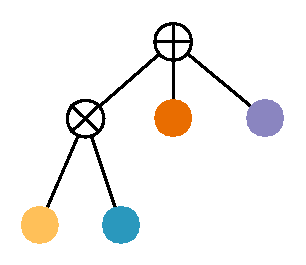
\includegraphics[width=0.24\linewidth]{figures/learnspn-2}&
  %   %     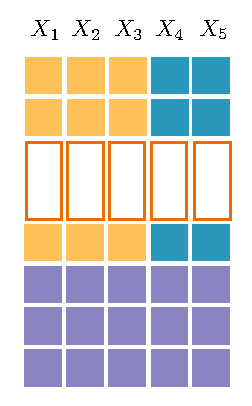
\includegraphics[width=0.208\linewidth]{figures/grid-3}&                                                          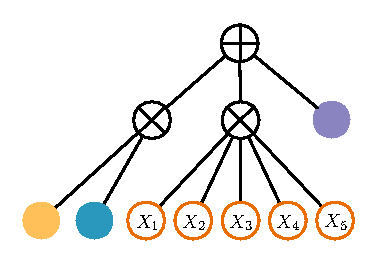
\includegraphics[width=0.30\linewidth]{figures/learnspn-3}\\                                             
  %   %   \end{tabular}
  %   % \end{table}
    
  % \end{textblock}
  
  
  \begin{textblock}{25.2}(54.8, 36.3)
    \footnotesize
    If there are less than $m$ instances, it puts a \textbf{\emph{naive
        factorization}} over leaves (Figure 1.d). For each univariate distribution
    it gets its \emph{\textbf{ML estimation}} smoothed by $\alpha$. LearnSPN
    hyperparameter space is thus: $\{\rho, \lambda, m, \alpha\}$.\par\bigskip
    
   %  \small
  %   \begin{itemize}
  % \item clustering instances with \textbf{\emph{online Hard-EM}} with cluster penalty
  %   $\lambda$:
  %   \[\begin{array}{cc}
  %       Pr(\mathbf{X})= \sum_{C_i \in \mathbf{C}}\prod_{X_j \in \mathbf{X}}Pr(X_j|C_i)Pr(C_i)\\
  %       % & Pr(C_i) \propto e^{-\lambda |\mathbf{C}|\cdot |\mathbf{X}|}\\
  %     \end{array}\]
  %     weights are the proportions of instances falling into each cluster
  %   \item if there are less than $m$ instances, put a \textbf{\emph{naive
  %         factorization}} over leaves
  %   \item each univariate distribution get \emph{\textbf{ML
  %         estimation}} smoothed by $\alpha$  
  %   \end{itemize}

    The state-of-the-art, in terms of test likelihood, is \textbf{ID-SPN}: it turns LearnSPN in log-likelihood guided expansion of sub-networks
    approximated by Arithmetic
    Circuits~\emph{\parencite{Rooshenas2014-short}}. However it is
    overparametrized, and slower.\par\bigskip
    
    
    Tractability is guaranteed if the network size is polynomial in \#
    vars. \emph{\textbf{Structure quality matters}} as much as likelihood. Comparing network sizes is more solid than comparing inference times.\par\bigskip

    LearnSPN is too greedy and the resulting SPNs are overcomplex
    networks that may not generalize well. \textbf{\emph{Structure quality desiderata}}: \emph{smaller} but \emph{accurate}, \emph{deeper} but not wider, SPNs. 
    
  \end{textblock}
  
  
  %
  % section 3
  \begin{textblock}{80}(0, 59.6)
    \usebeamerfont{section name}
    Random query embedding extraction
  \end{textblock}
  
  % 
  % % section 3.1
  % \begin{textblock}{20}(54.8, 59.6)
  %   \usebeamerfont{section name}
  %   Experiments
  % \end{textblock}
  
  \begin{textblock}{25.2}(0, 62.1)
    \footnotesize
    \setlength{\leftmargini}{30pt}
    \textsf{LearSPN} performs two interleaved \textbf{\emph{greedy
        hierarchical}} divisive \textbf{\emph{clustering}}
    processes. Each process benefits from the other one improvements
    and similarly suffers
    from the other's mistakes.\par\bigskip
    
    \textbf{Idea}: slowing down the processes by limiting the number of
    nodes to split into. \textsf{SPN-B}, variant of \textsf{LearnSPN} that uses EM
    for mixture modeling but doing only \textsf{B}inary splits for sum nodes children
    ($k=2$) when clustering rows.\par\bigskip
    
    \raisebox{55pt}{\begin{minipage}[t]{0.6\linewidth}
        \flushleft
    %  Objectives:
    %   \begin{itemize}
    %   \item not committing to complex structures too early  
    %   \item same expressive power: successive row splits can represent
    %     sum nodes with more than two children
    %   \item reducing node out fan increases the network depth 
    %   %\item same accuracy, smaller networks
    %   \end{itemize}
    % \end{minipage}}\hfill\begin{minipage}[c]{0.35\linewidth}
    %   \begin{center}
    %     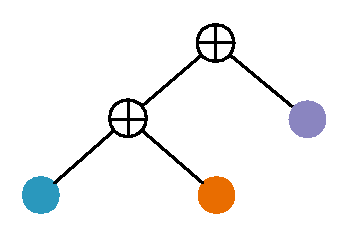
\includegraphics[width=0.85\linewidth]{figures/learnspn-4}
    %   \end{center}
    % \end{minipage}
    \textbf{Objectives}: not committing to complex structures too early while
    retaining same expressive power (right Figure is equivalent to the
    SPN in Figure 1.b); moreover, reducing
          the node out fan increases the network depth. Plus, there is no
          need for $\lambda$ anymore.
      \end{minipage}}\hspace{40pt}\begin{minipage}[c]{0.3\linewidth}
      \begin{center}
        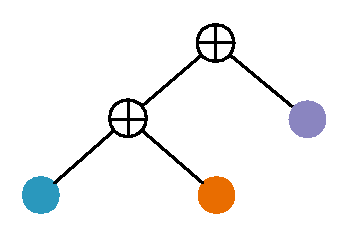
\includegraphics[width=7.5cm]{figures/learnspn-4}
      \end{center}
    \end{minipage}
      \end{textblock}
  
   \begin{textblock}{25.2}(27.4, 62.1)
        \footnotesize
    % \begin{algorithm}[H]
    %   \caption{\textsf{randQueryEmbedding}($\mathcal{D}$, $k$)}
    %   \label{algo:randQuery}
      \begin{algorithmic}[1]
        \State \textbf{Input:} a set of instances
        $\mathcal{D}=\{\mathbf{x}^{i}\}_{i=1}^{m}$ over r.v.s
        $\mathbf{X}=\{X_1,\dots,X_n\}$, $k$ as the number of features to generate
        \State  \textbf{Output:}  a set of embeddings
        $\mathcal{E}=\{\mathbf{e}^{i}\}_{i=1}^{m}, \mathbf{e}^{i}\in\mathbb{R}^{k}$
        
        \State $\theta\leftarrow\mathsf{learnDensityEstimator}(\mathcal{D})$
        \State $\mathcal{E}\leftarrow\{\}$
        \For {$j=1,\dots,k$}
        \State $\mathbf{Q}_{j}\leftarrow \mathsf{selectRandomRVs}(\mathbf{X})$
        \For {$i=1,\dots,m$}
        \State $e^{i}_{j}= p_{\theta}(\mathbf{x}^{i}_{\mathbf{Q}_{j}})$  
        \EndFor
        \State $\mathcal{E}\leftarrow\mathcal{E}\cup\{\mathbf{e}^{i}\}$
        \EndFor
        \Return {$\mathcal{E}$}
      \end{algorithmic}
    %\end{algorithm}
  \end{textblock}
  
  \begin{textblock}{25.2}(54.8, 62.1)
    \footnotesize
    % \begin{algorithm}[!t]
    %   \caption{\textsf{randPatchEmbedding}($\mathcal{D}$, $s$, $d$)}
    %   \label{algo:randPatch}
      \begin{algorithmic}[1]
        \State \textbf{Input:} a set of instances
        $\mathcal{D}=\{\mathbf{x}^{i}\}_{i=1}^{m}$ over r.v.s
        $\mathbf{X}=\{X_1,\dots,X_n\}$,
        $s$ as the number of patches to extract,
        $d$ as the patch length,
        \State  \textbf{Output:}  a set of embeddings
        $\mathcal{E}=\{\mathbf{e}^{i}\}_{i=1}^{m}, \mathbf{e}^{i}\in\mathbb{R}^{k}$
        \State $\mathcal{R}\leftarrow\{\}$
        \For {$i=1,\dots,s$}
        \State $\mathbf{x}^{\mathsf{rand}}\leftarrow
        \mathsf{selectRandomSample}(\mathcal{D})$
        \State $\mathbf{r}^{i}\leftarrow
        \mathsf{extractRandomPatch}(\mathbf{x}^{\mathsf{rand}}, d)$
        \State $\mathcal{R}\leftarrow\mathcal{R}\cup\{\mathbf{r}^{i}\}$
        \EndFor
        
        \State $\theta\leftarrow\mathsf{learnDensityEstimator}(\mathcal{R})$

        \State $\mathcal{E}\leftarrow\{\}$
        \For {$i=1,\dots,m$}
        \State $j\leftarrow 0$
        \For {\textbf{each} patch $\mathbf{q}^{i}, |\mathbf{q}^{i}|=d$ in
          $\mathbf{x}^{i}$}
        \State $e^{i}_{j}= p_{\theta}(\mathbf{q}^{i})$
        \State $j\leftarrow j + 1$
        \EndFor
        \State $\mathcal{E}\leftarrow\mathcal{E}\cup\{\mathbf{e}^{i}\}$
        \EndFor
        \Return {$\mathcal{E}$}
      \end{algorithmic}
      %\end{algorithm}
      \end{textblock}
      

        
  % % 
  % % section 4
  % \begin{textblock}{80}(0, 66.6)
  %   \usebeamerfont{section name}
  %   Regularizing by introducing tree distributions as leaves
  % \end{textblock}
  
  % \begin{textblock}{25.2}(0, 69.1)
  %   \footnotesize
  %   LearnSPN regularization is is governed by the hyperparameters $\alpha$ and $m$,
  %   however using naive factorizations can be ineffective. In order to
  %   get accurate networks, the algorithm prefers smaller values for
  %   $m$, resulting in more complex networks\par\bigskip
    
  %   \textbf{Idea}: substitute naive factorizations with Bayesian trees as
  %   \emph{\textbf{multivariate tractable tree
  %       distributions}}. \textsf{SPN-BT} learns such \textsf{T}rees
  %   with the Chow-Liu algorithm when stopping the splitting process.\par\bigskip

  %   \begin{minipage}[t]{0.6\linewidth}
  %       \flushleft
  %       \textbf{Objectives}: represent more information allowing for larger
  %       values of $m$ to be chosen, while preserving tractability for marginals,
  %       conditionals and MPE inference\\(still linear in the number of leaves).
  %     \end{minipage}% \hspace{40pt}\begin{minipage}[c]{0.3\linewidth}
  %   %   \hspace{-30pt}
  %   %    %\begin{center}
  %   %     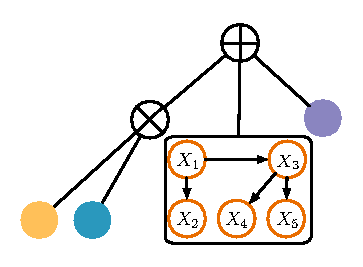
\includegraphics[width=8.2cm]{figures/spn-clt}
  %   %   %\end{center}
  %   % \end{minipage}
  % \end{textblock}

  % \begin{textblock}{10}(15.8, 76.1)
  %   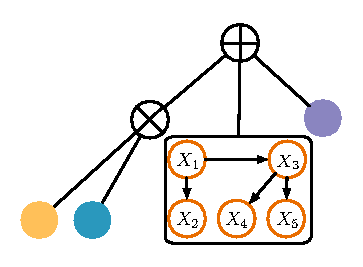
\includegraphics[width=8.2cm]{figures/spn-clt}
  %   \end{textblock}
  
  % \begin{textblock}{25.2}(27.4, 69.1)
  %   \footnotesize
  %   \textsf{SPN-BT} reduces the
  %   size of the networks even more while preserving \textsf{SPN-B}
  %   accuracy. At larger values of $m$, when both \textsf{SPN-B} and \textsf{LearnSPN}
  %   accuracies tend to decrease, \textsf{SPN-BT} seems to preserve or
  %   improve its likelihood.
      
  %   \begin{center}
  %     \begin{table}[ht]
  %       \setlength{\tabcolsep}{30pt}  
  %       \begin{tabular}{c c}
  %         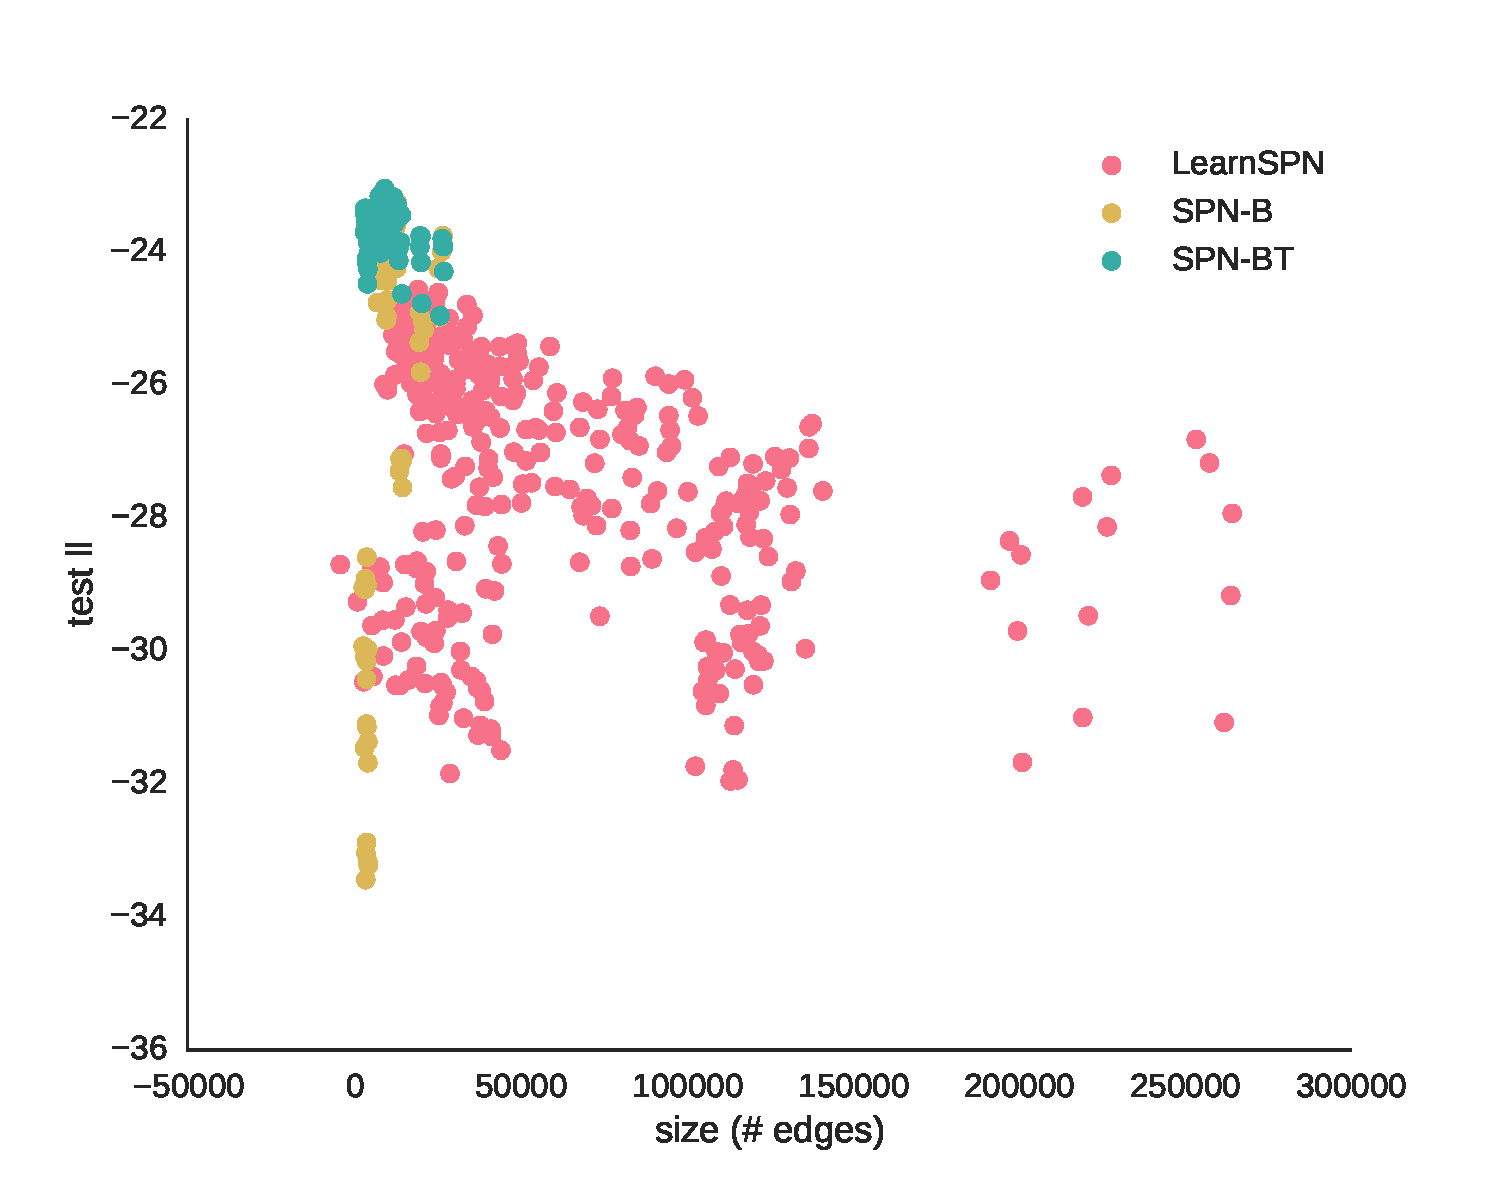
\includegraphics[width=0.4\linewidth]{figures/ll-depth/10-8/pumsb-star-ll-depth}&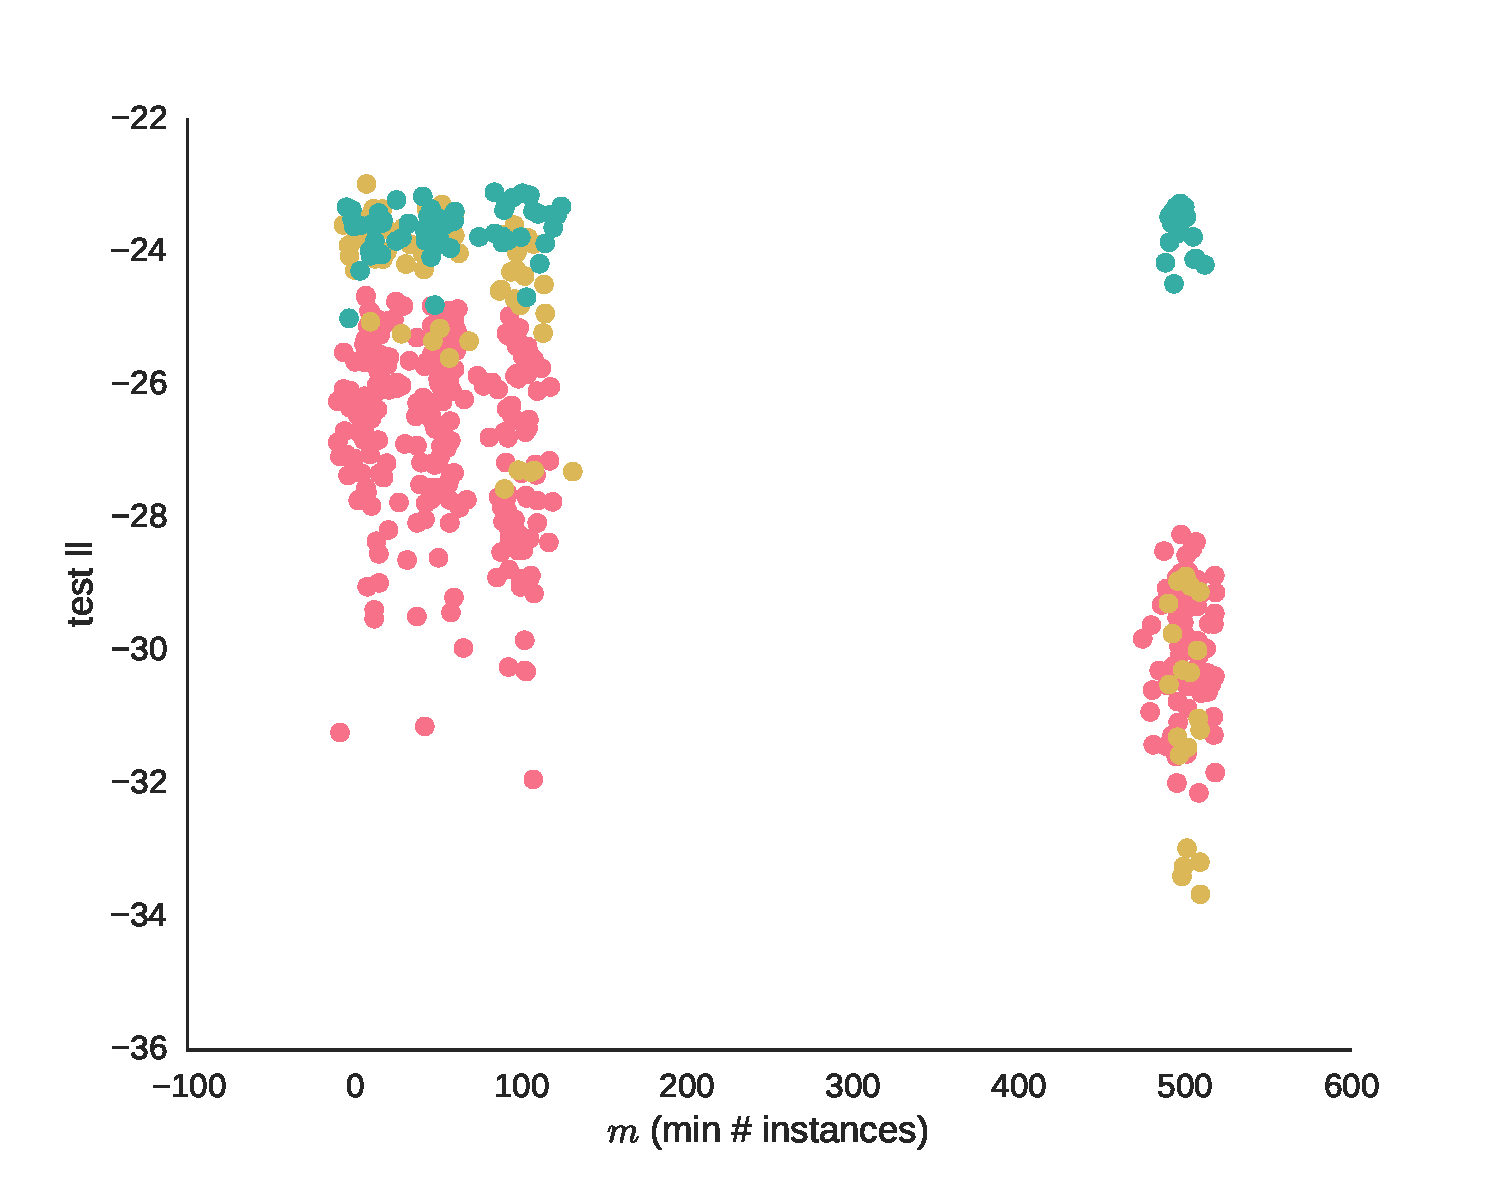
\includegraphics[width=0.4\linewidth]{figures/ll-m/10-8/pumsb-star-ll-m}
  %       \end{tabular}
  %     \end{table}
  %   \end{center}
    
  %   \vspace{-20pt}
  %   \begin{center}
  %     \begin{minipage}[t]{0.9\linewidth}
  %       \tiny\flushleft
  %       Figure 3. Comparing network sizes (left) and values for $m$
  %       against the  average test
  %       log-likelihood obtained by \textsf{LearnSPN}, \textsf{SPN-B} and
  %       \textsf{SPN-BT}
  %       number of sum node children splits. Each dot is an experiment
  %       in the grid search performed for the dataset Pumsb-star.
  %     \end{minipage}
  %   \end{center}

  % \end{textblock}
  
  % \begin{textblock}{25.2}(54.2, 68.4)
  %   \small
  %   \blindtext
  % \end{textblock}
      
  
  % 
  % section 5
  \begin{textblock}{80}(0, 82.9)
    \usebeamerfont{section name}
    Evaluation
  \end{textblock}
  
  \begin{textblock}{25.2}(0, 85.4)
    \small
    Empirical evaluation of the random marginal query approach:
    \begin{itemize}
    \item 5 binary image datasets: rectangles (\textsf{REC}),
      convex (\textsf{CON}), ocr\_letters (\textsf{OCR}), caltech101
      (\textsf{CAL}), binary MNIST (\textsf{BMN})
    \item  OVR L2-reg logistic regressor for all representations, \textsf{LR}
      baseline  
    \end{itemize}
  \end{textblock}
  
  \begin{textblock}{25.2}(27.4, 85.4)
    \small
    \begin{itemize}
    \item 3 SPN models trained with
      \textsf{LearnSPN-b}~\parencite{Vergari2015} with $m\in\{500,
      100, 50\}$  (\textsf{SPN-I}, \textsf{SPN-II}, \textsf{SPN-III})
    \item 3 Mixture of trees models with $k\in\{3,15,30\}$
      (\textsf{MT-I}, \textsf{MT-II}, \textsf{MT-III})
    \end{itemize}
  \end{textblock}
  
  \begin{textblock}{25.2}(54.8, 85.4)
    \small
    \begin{itemize}
    \item 1000 randomly generated marginal queries corresponding to
      adjacent pixels in a rectangular image patch having minimum sizes of 2
      pixels and maximum of 7 pixels for \textsf{OCR} and 10 pixels for the
      remaining datasets
    \end{itemize}
  \end{textblock}
  
  \begin{textblock}{80}(0, 90.8)
    \begin{center}
      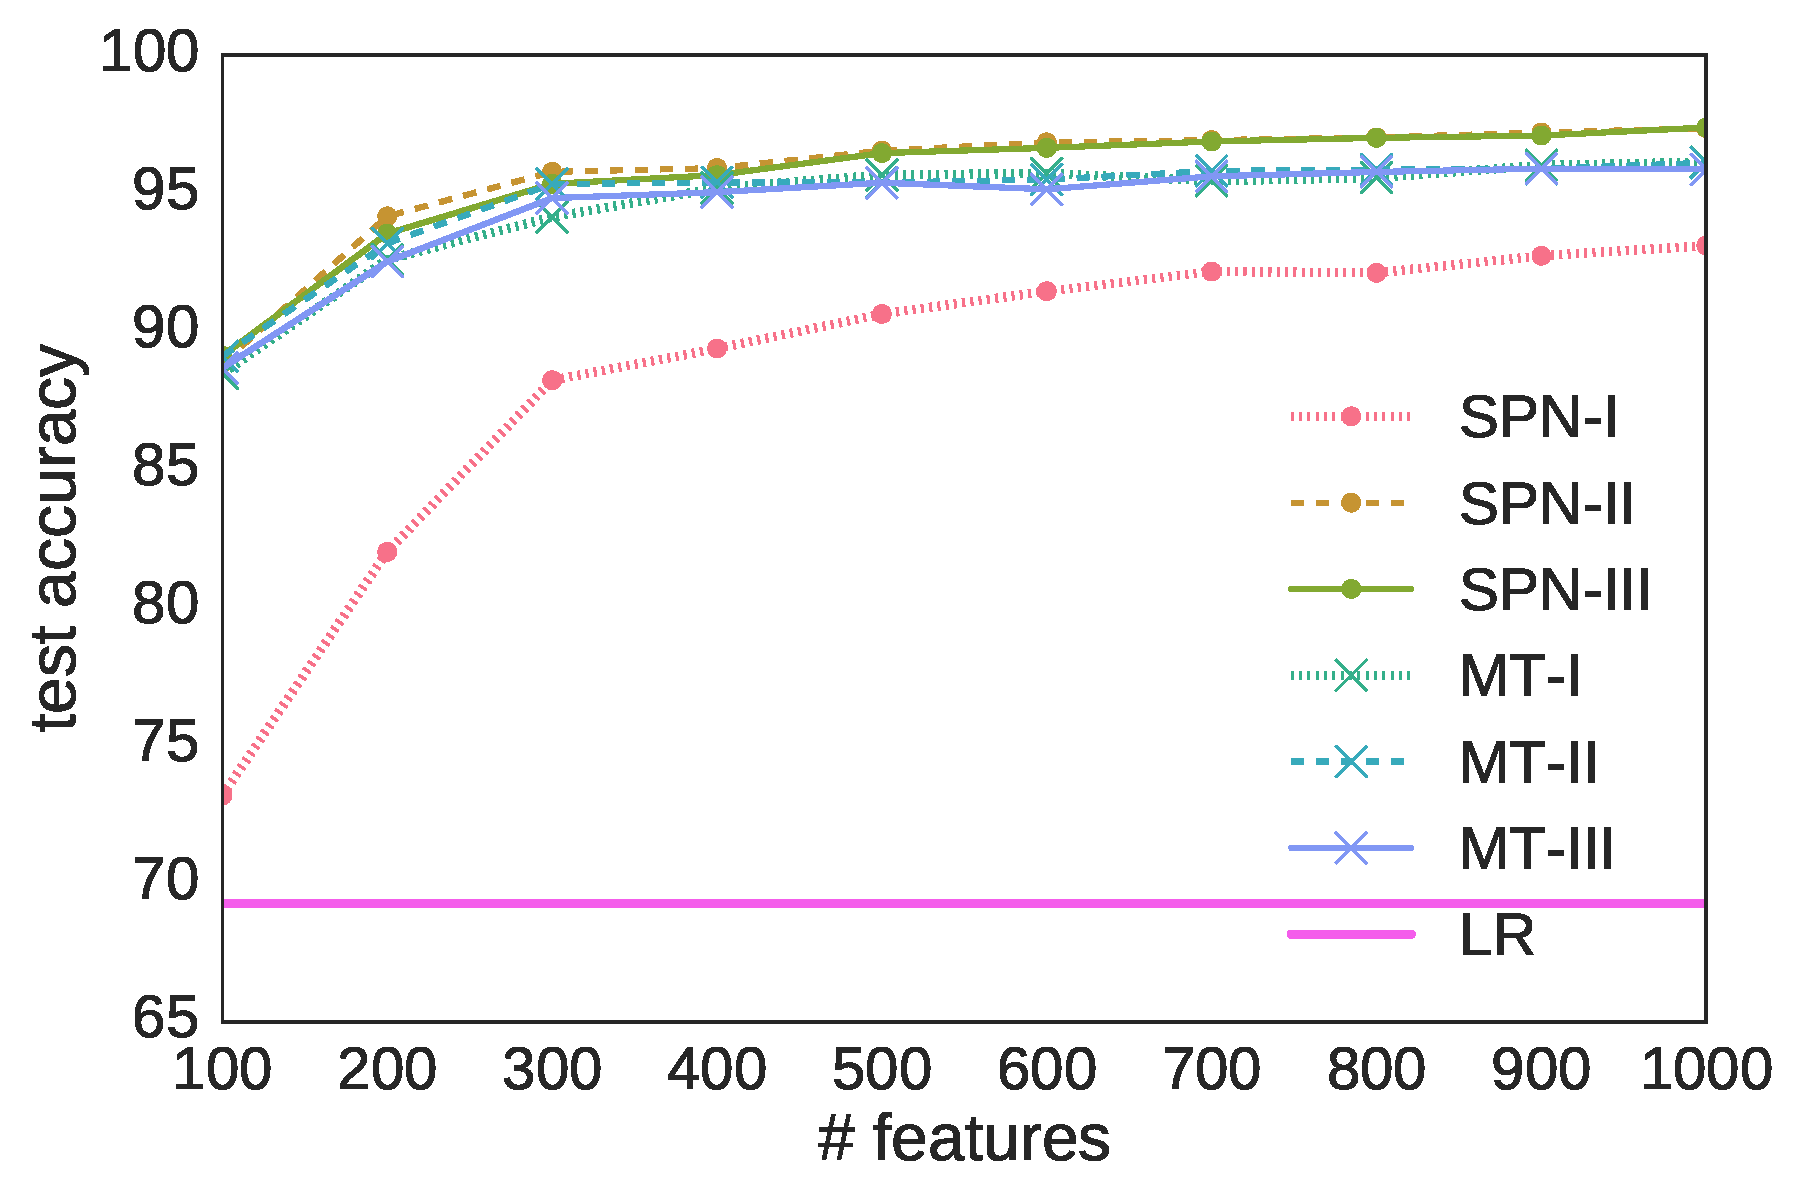
\includegraphics[width=0.2\columnwidth]{figures/lines-rectangles}
      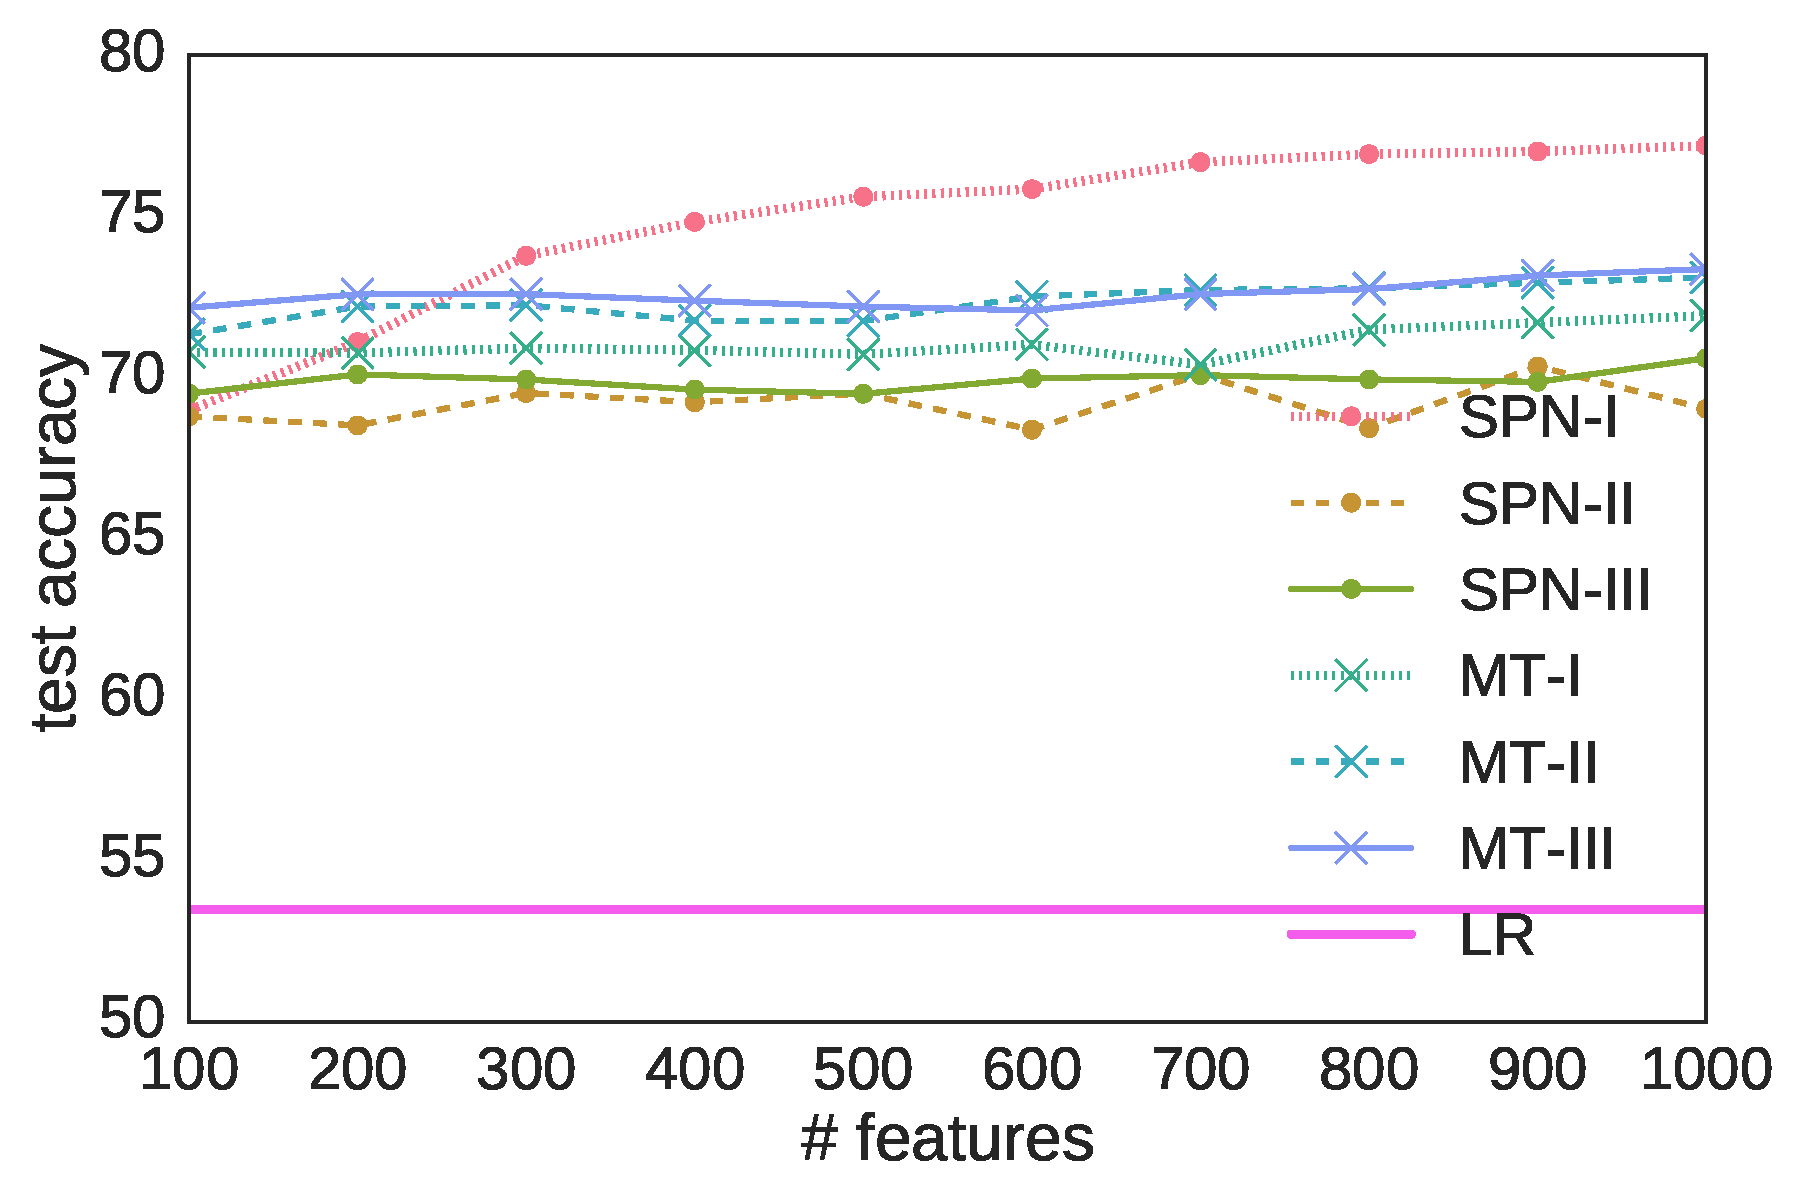
\includegraphics[width=0.2\columnwidth]{figures/lines-convex}
      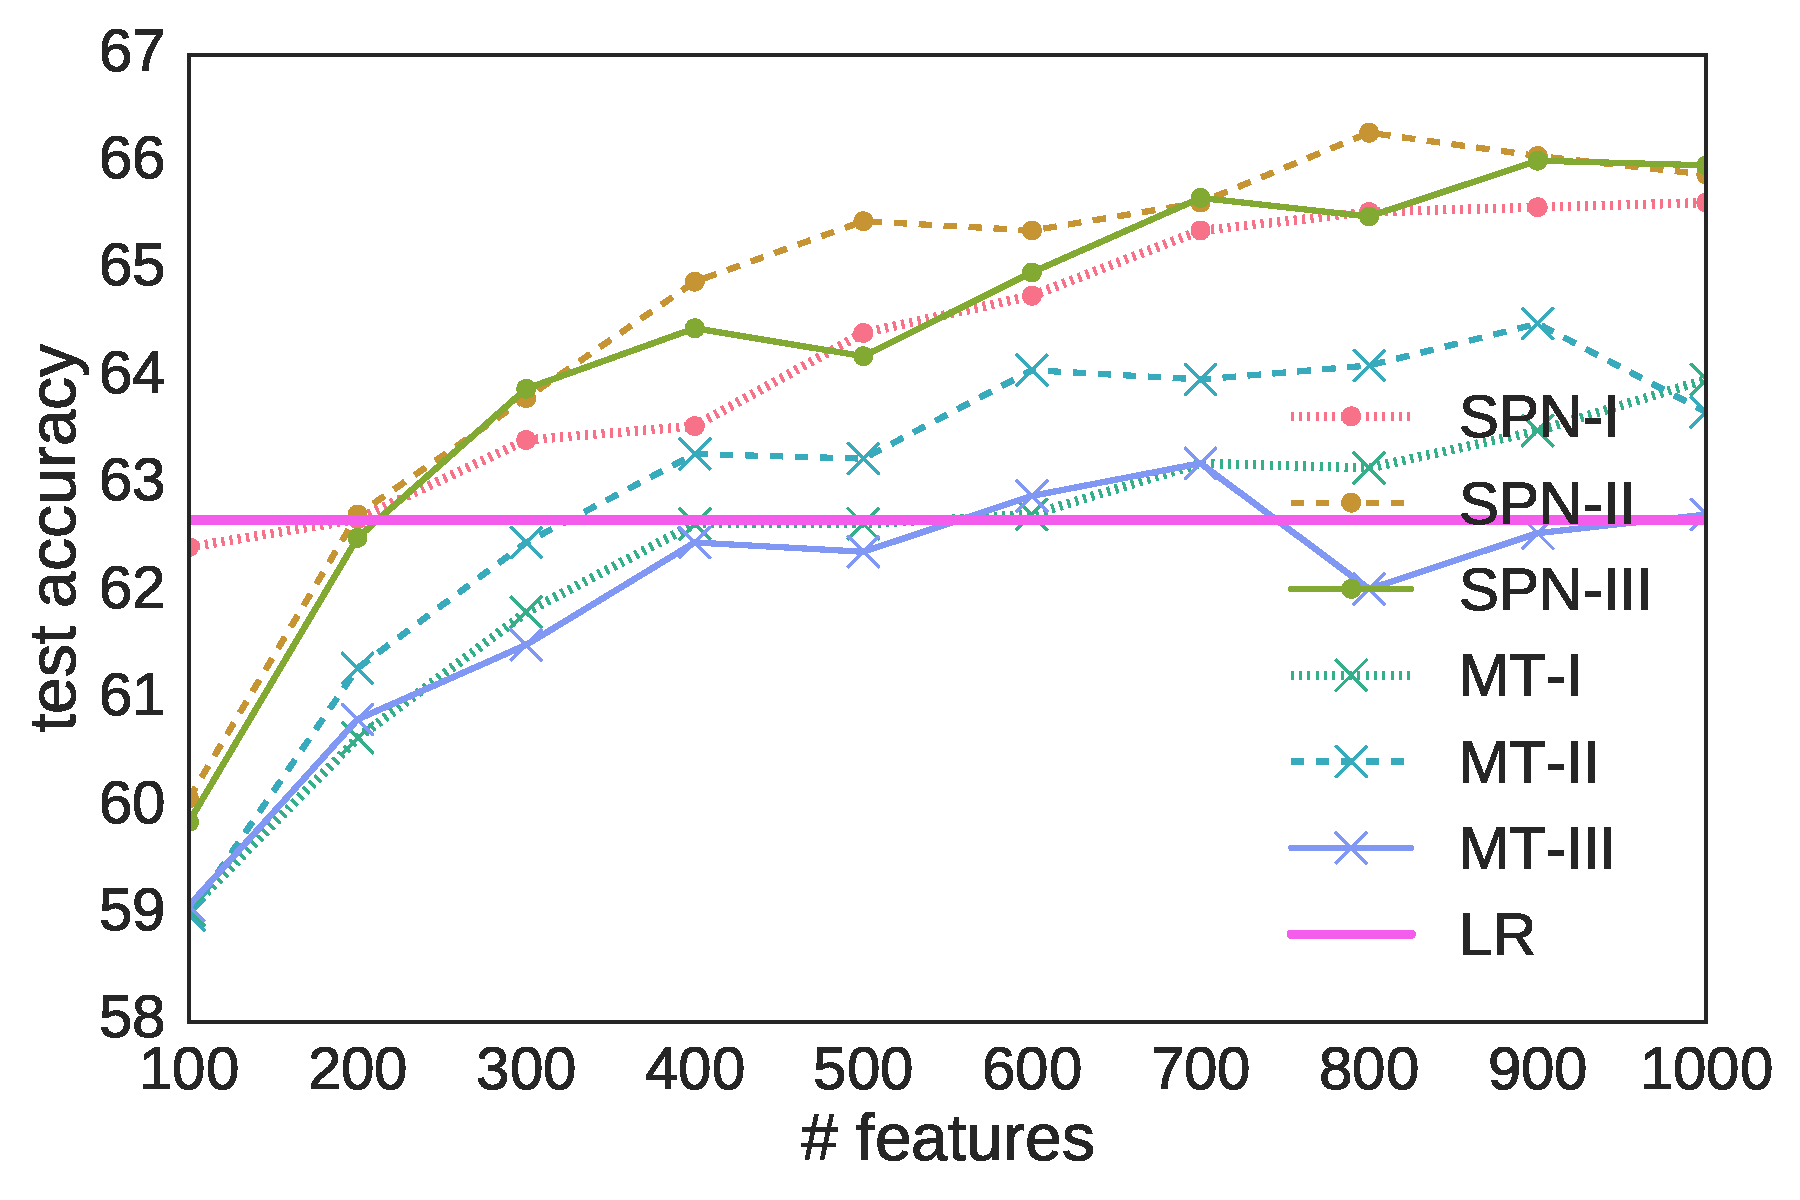
\includegraphics[width=0.2\columnwidth]{figures/lines-caltech101}
      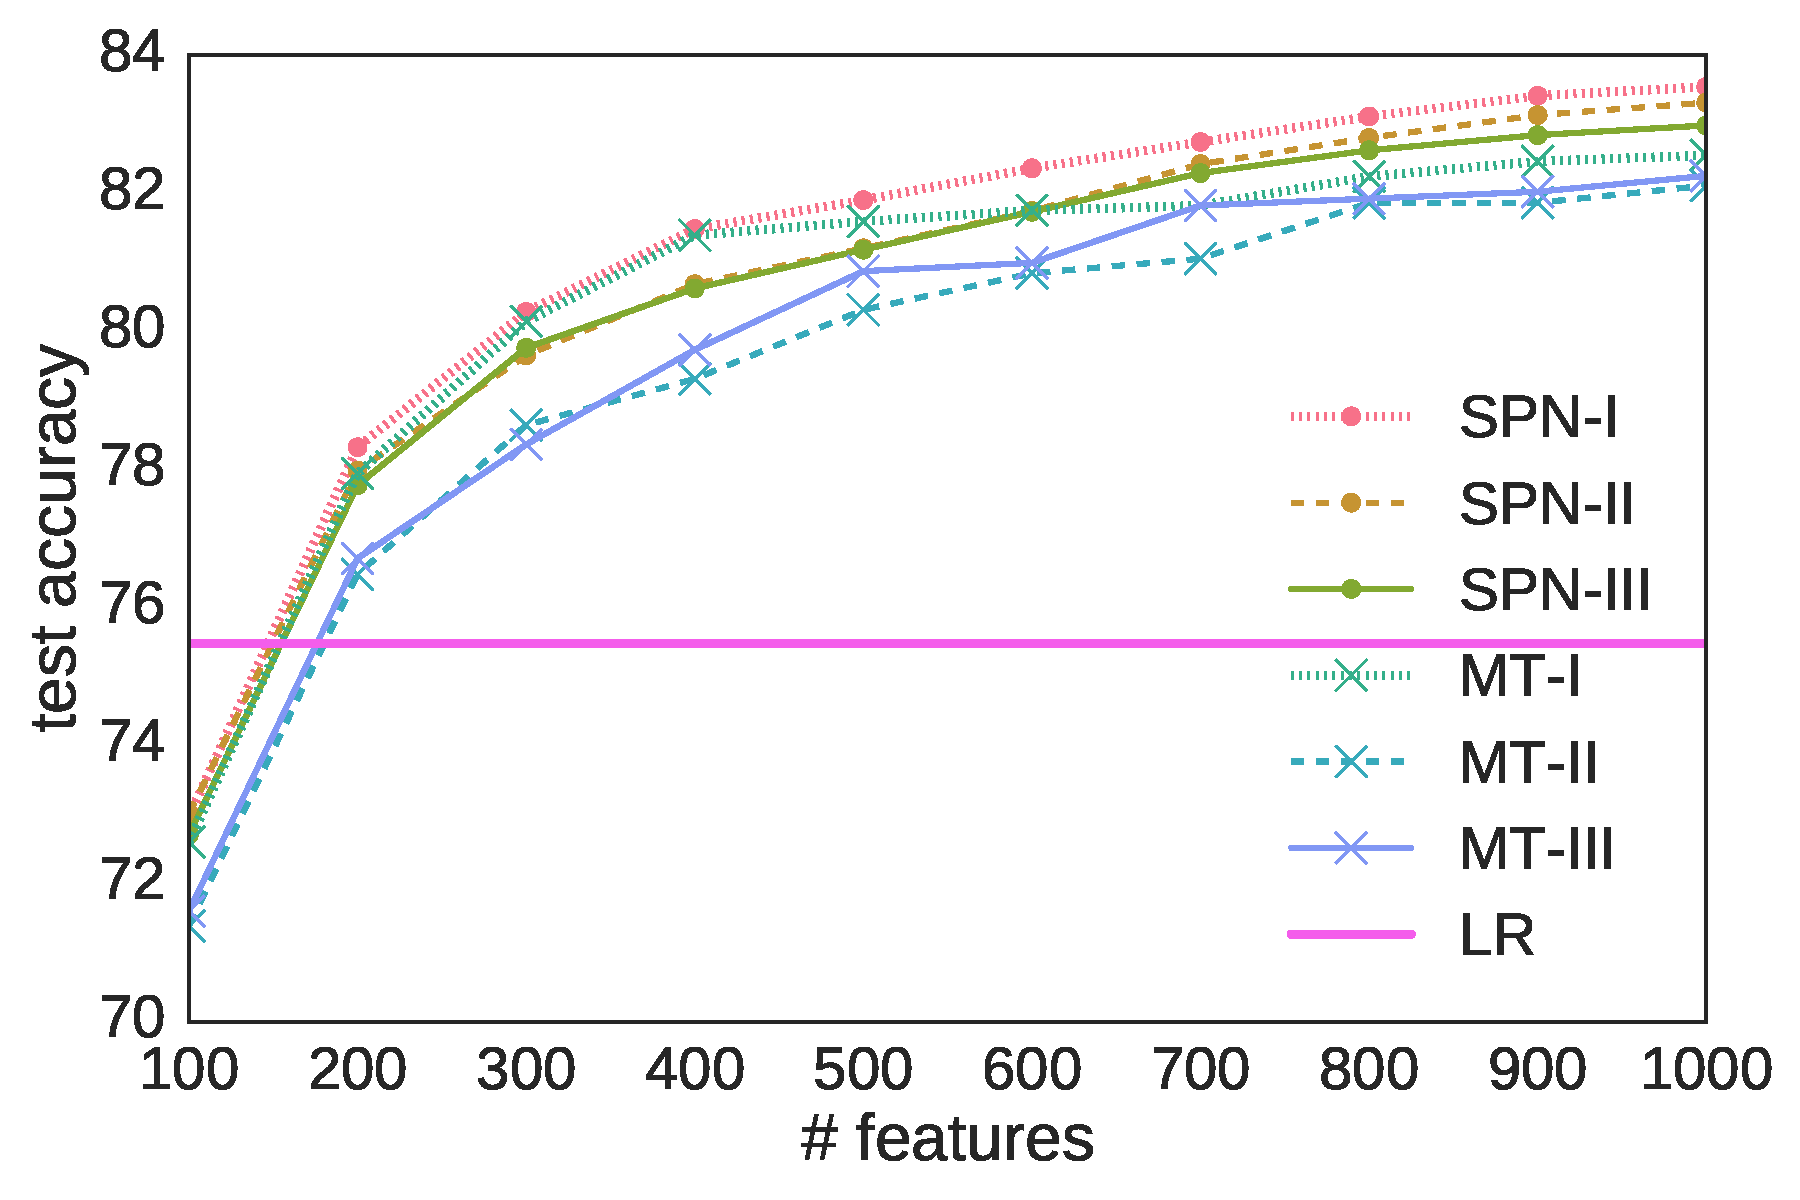
\includegraphics[width=0.2\columnwidth]{figures/lines-ocr_letters}
      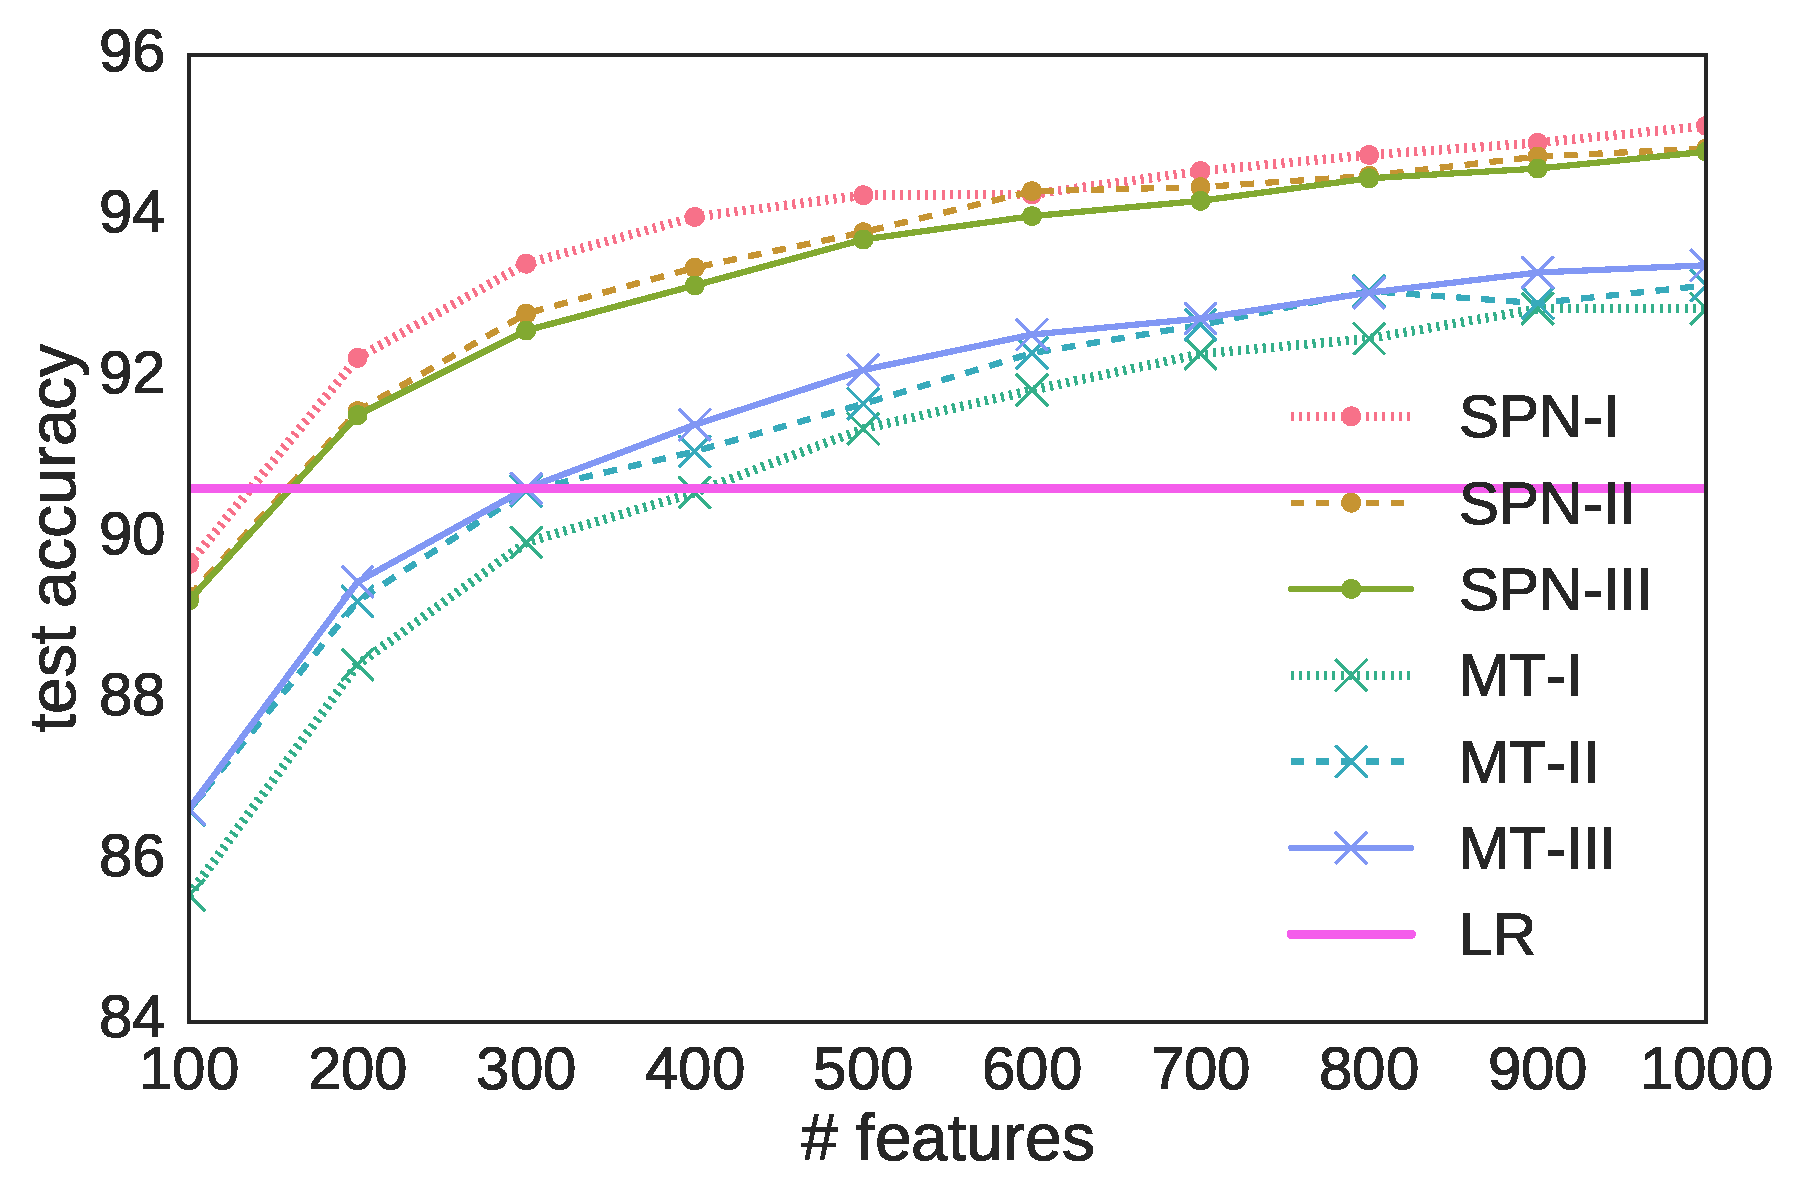
\includegraphics[width=0.2\columnwidth]{figures/lines-bmnist}
    \end{center}
  \end{textblock}
  
  % 
  % section 5
  \begin{textblock}{80}(0, 104.)
    \usebeamerfont{section name}
    References
  \end{textblock}

  
 \begin{textblock}{52}(0, 106.5)
    \small
    % \blindtext
    \setlength\bibitemsep{8pt}
    \printbibliography[heading=none]
  \end{textblock}
  
  \begin{textblock}{25.2}(27.4, 106.5)
    \small
    % \blindtext
  \end{textblock}
  
  % \begin{textblock}{25.2}(54.2, 105.8)
  %   \small
  %   % \blindtext
  % \end{textblock}

  % 
  % footer
  \begin{textblock}{80}(0, 114.3)
    \usebeamerfont{subtitle}
    \footnotesize
    \textbf{ECML-PKDD 2016}  -  19th-23rd September 2016, Riva del Garda, Italy\hfill
  \end{textblock}
  
\end{frame}




\end{document}

%%% Local Variables:
%%% mode: latex
%%% TeX-master: t
%%% TeX-engine: xetex
%%% End:
